\documentclass{article}

\usepackage[utf8]{inputenc}
\usepackage[french]{babel}

\usepackage{hyperref}
\usepackage{graphicx}
\graphicspath{ {./resources/} }

\author{
    Valentin Jonquière,
    Mathilde Chollon
}

\title{Rapport Projet Approche Objet}

\begin{document}

\maketitle

\pagebreak

\tableofcontents

\pagebreak

\section{Contributions}
Le travail a été réparti sous forme de 'taches' ce qui nous a permis de toucher à tous les composants de notre application
et de ne pas limiter une personne au développement du \textit{controller} pas exemple. Nous avons également passé beaucoup
de temps à réfléchir à l'architecture des classes, les design pattern à employer que nous avons renseignés dans un diagramme
UML avant de commencer à coder l'application.

\section{Structure de code}
Nous avons choisi d'utiliser une architecture \textit{MVC} et de donc diviser notre application dans trois grands packages: \textit{Model}, \textit{View}
et \textit{Controller}. À l'interieur de ces packages, nous avons parfois dû regrouper des ensembles de classes dans d'autres sous-packages pour rendre
la structure de l'application plus simple. C'est pour cela que l'on retrouve un package \textit{Building} regroupant toutes les classes relatives
aux bâtiments (le décorateur, leur gestion, ...). Nous avons créé un diagramme des classes UML complet que vous pouvez retrouver ci-dessous.

\begin{figure}[h]
    \caption{Diagramme des classes général}
    \centering
    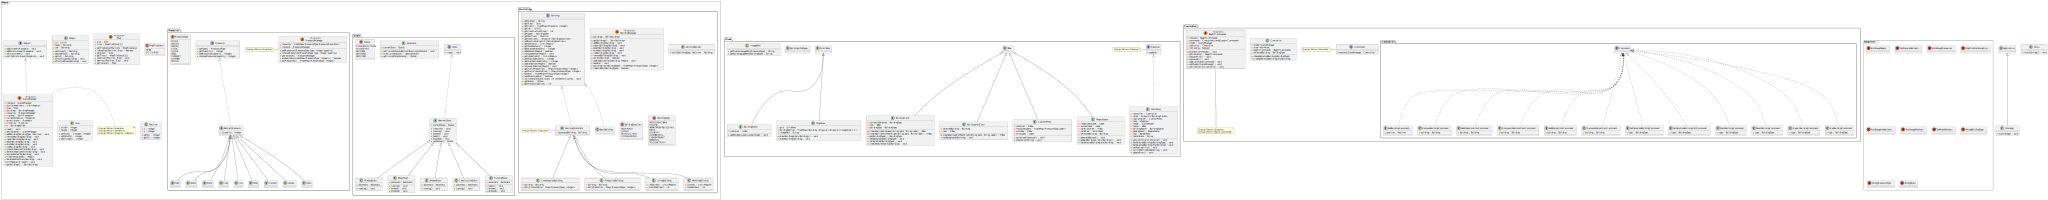
\includegraphics[width=\textwidth,height=\textheight,keepaspectratio]{complete_UML}
    \label{fig:UML_complet}
\end{figure}


Celui-ci étant trop étendu pour bien distinguer toutes les classes, voici un découpage par les principaux packages (\textit{Model}, \textit{View}, \textit{Controller}).

\begin{figure}[h]
    \caption{Diagramme des classes package controller}
    \centering
    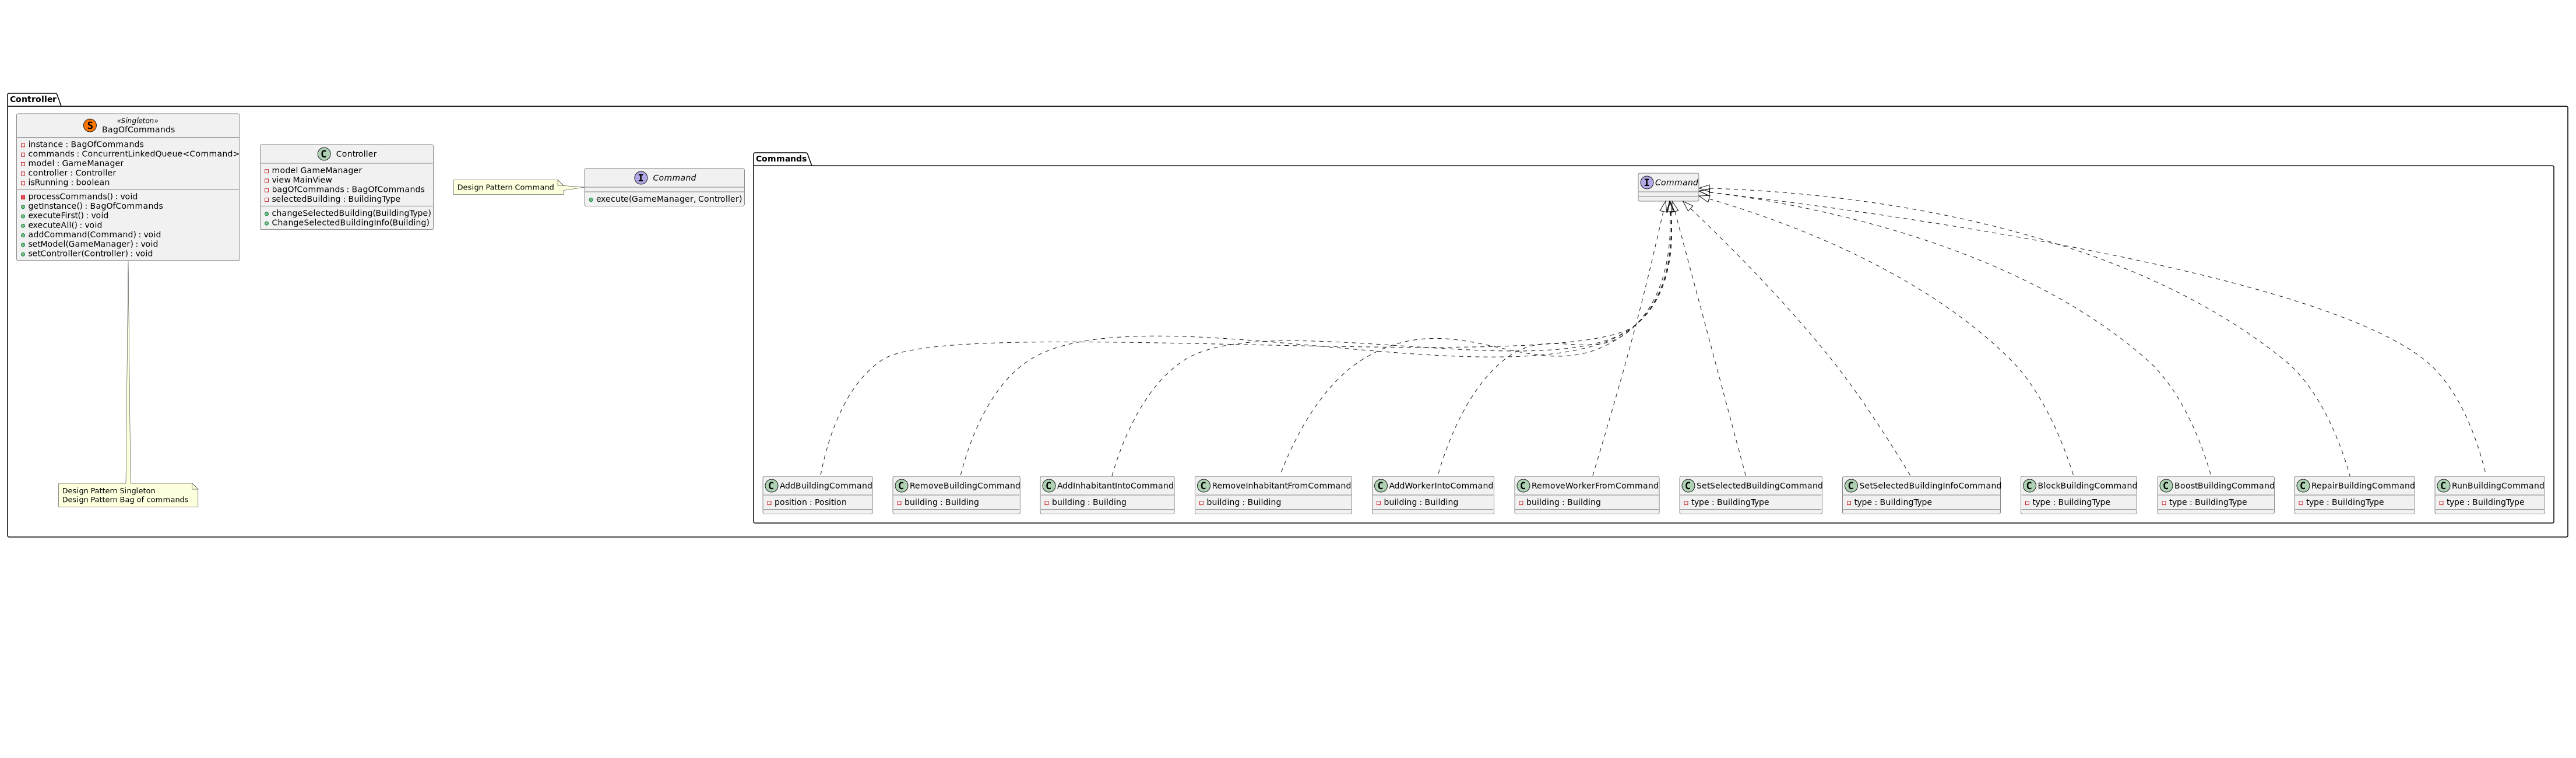
\includegraphics[width=\textwidth,height=\textheight,keepaspectratio]{controller_UML}
    \label{fig:UML_complet}
\end{figure}
\pagebreak
\begin{figure}[h]
    \caption{Diagramme des classes package model}
    \centering
    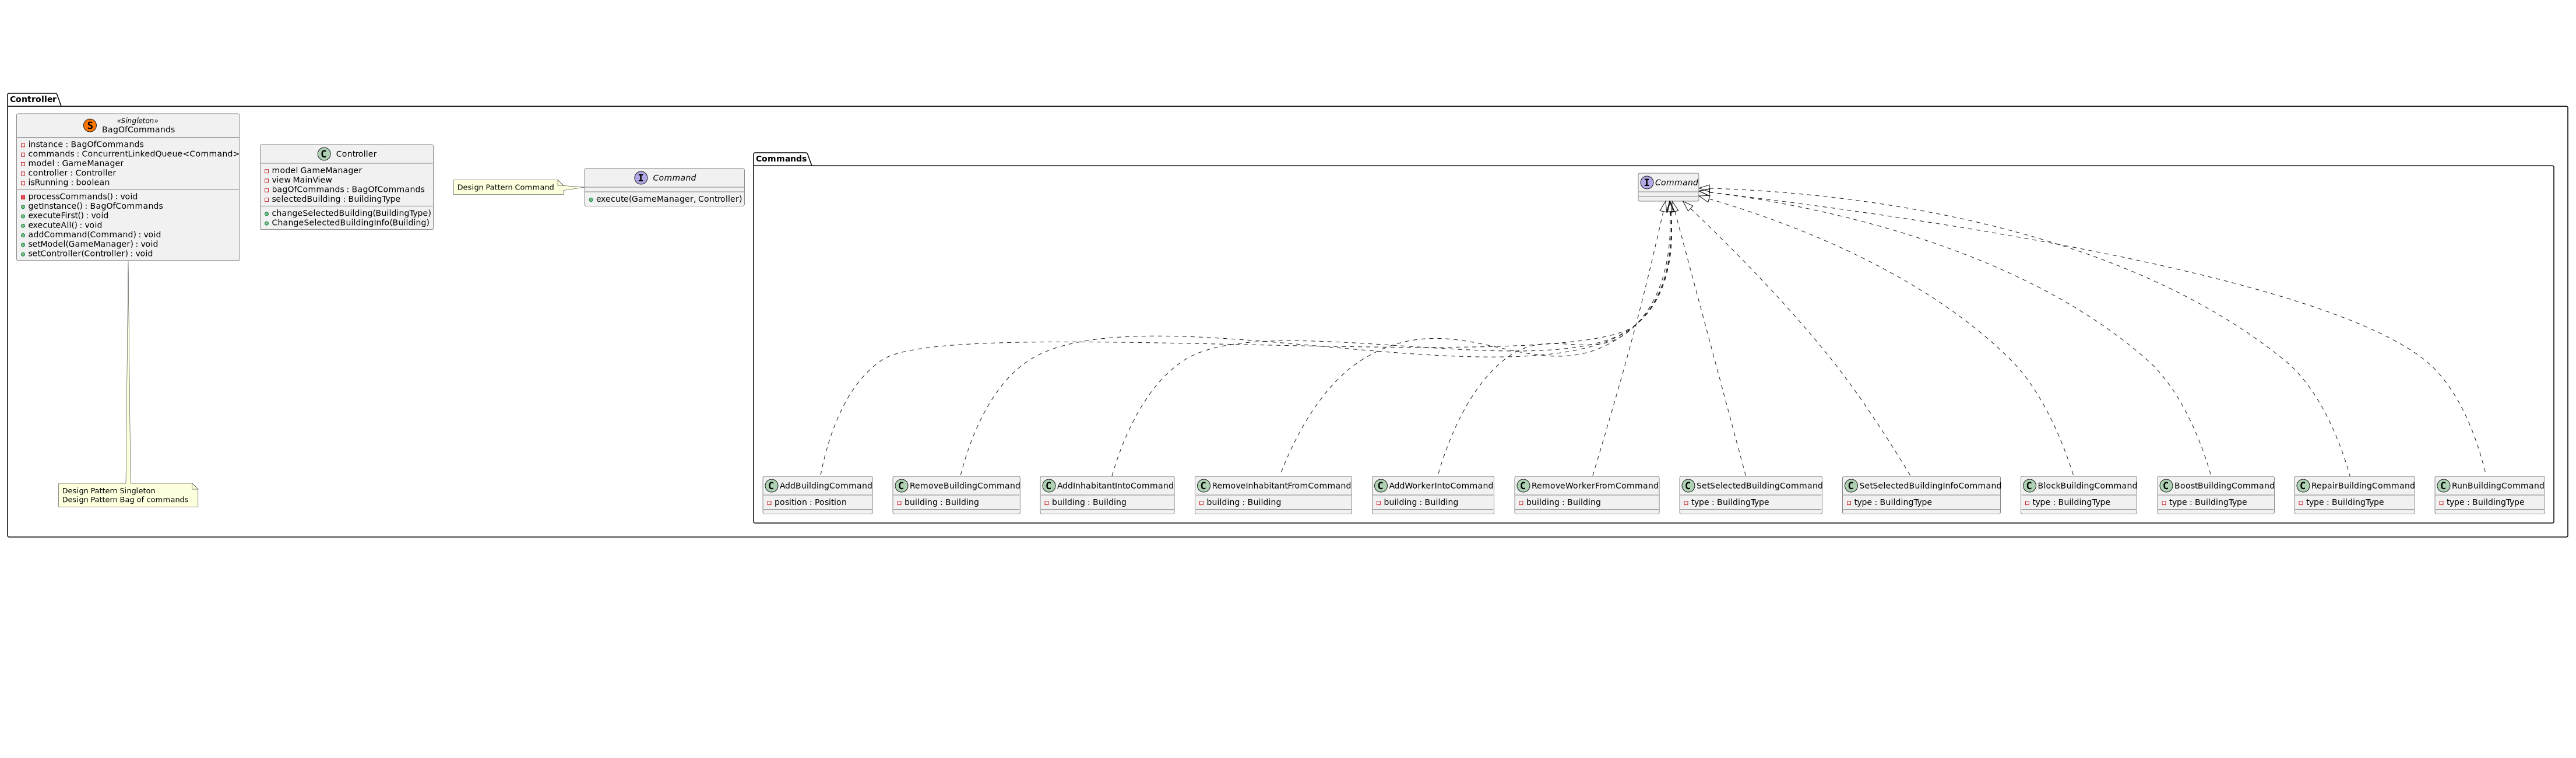
\includegraphics[width=\textwidth,height=\textheight,keepaspectratio]{controller_UML}
    \label{fig:UML_complet}
\end{figure}
\pagebreak

\begin{figure}[h]
    \caption{Diagramme des classes package view}
    \centering
    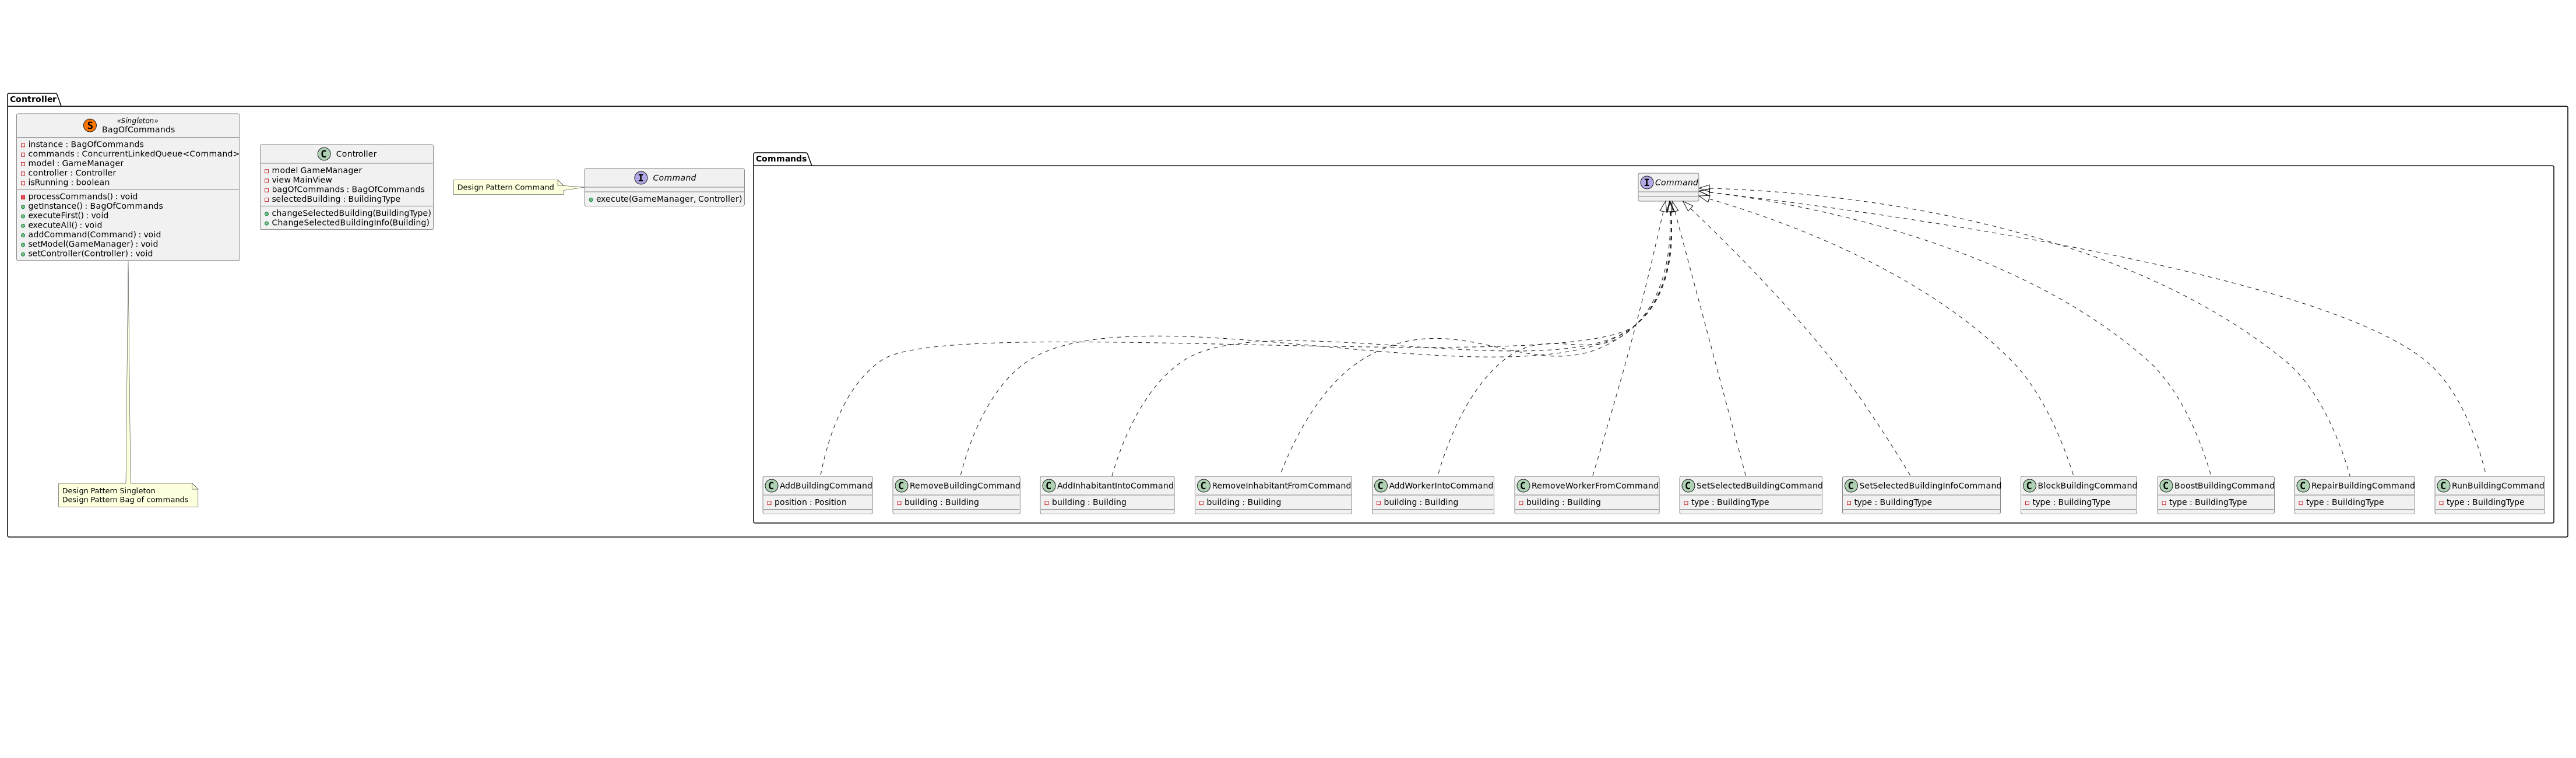
\includegraphics[width=\textwidth,height=\textheight,keepaspectratio]{controller_UML}
    \label{fig:UML_complet}
\end{figure}
\pagebreak
\pagebreak

\section{Design pattern}
\subsection{Decorator}
Nous avons utilisé le design pattern decorator afin de rendre plus simple l'ajout de nouveaux bâtiments.
En effet, nous avons vite distingué qu'il y avait seulement 4 fonctions pour les bâtiments:
\begin{itemize}
    \item Avoir des travailleurs
    \item Avoir des habitants
    \item Générer des ressources
    \item Consommer des ressources
\end{itemize}
Tous les bâtiments possédant au moins une de ces caractéristiques nous avons créé les 4 décorateurs correspondants
(qui nous permettent d'intégrer tous ceux du sujet). L'utilisation de ce design pattern rend ainsi l'intégration
d'un nouveau type de bâtiment immédiat (il n'y a pas besoin de créer de classes compliquées, mais uniquement de choisir
si l'on veut qu'il puisse accueillir des habitants par exemple). Le point fort de ce design pattern et qu'il nous permet
de ne pas à avoir à se soucier de savoir si un bâtiment doit produire des ressources par exemple, et de devoir stocker les
bâtiments en plusieurs exemplaires. En effet, ils sont tous de type \textit{Building} avec pour chacun ses spécificités.

\subsection{Builder}
Pour venir compléter le design pattern \textit{Decorator} et rendre les bâtiments modulaires nous avons utilisé le design
pattern builder pour associer les bons décorateurs aux bâtiments que l'on souhaite construire. C'est ici le rôle de la
classe \textit{BuildingBuilder} qui avec uniquement le type du bâtiment voulu (\textit{WoodenCabin}, \textit{Factory}), 
nous permet d'obtenir un bâtiment bien formé (avec sa consommation, production, nombre d'habitants et de travailleurs bien 
initialisés). Le builder rend la création de bâtiment simple (pas besoin de chercher les paramètres à chaque fois) et permet 
d'ajouter un nouveau type en ne le définissant qu'une seule fois.

\subsection{Observer/Listener}
Nous avons utilisé le design pattern \textit{Observer} sous sa forme \textit{Listener} afin de pouvoir mettre à jour automatiquement
notre vu lors d'un changement du modèle. Ceci casse l'architecture traditionnelle du \textit{MVC} mais évite d'avoir un \textit{Controller}
redondant de manière 'inutile'. Afin de traiter les traiter les erreurs montrées à l'utilisateur différemment, nous avons mis en place
un second \textit{Listener} spécifique aux erreurs, notamment car nous avons créé plusieurs exceptions spécifiques que l'on intercepte
dans le model (classe \textit{GameManager}) et que l'on peut faire remonter à l'utilisateur par l'intermédiaire de la vue.

\subsection{State}
En voyant que les buildings devaient avoir un temps de construction avant d'être opérationnels, nous avons pensé qu'un design pattern
\textit{State} était une bonne solution. Pour que celui-ci ait plus d'intérêt, nous avons décidé d'ajouter plusieurs autres états possibles
pour un bâtiments.
\begin{itemize}
    \item Construction: état de base lorsque l'on construit un bâtiment (initial state)
    \item Running: le bâtiment fait ses actions normales tels que générer/consommer des ressources
    \item Blocked: le bâtiment est mis en 'pause', il ne génère/consomme plus de ressources
    \item Boosted: le bâtiment produit deux fois plus de ressources pendant un temps donné
    \item Broken: le bâtiment ne produit plus de ressources à moins d'être réparé
\end{itemize}

\subsection{MVC}
Nous avons utilisé l'architecture \textit{MVC} pour structurer notre application. Nous avons séparé les 3 principales composantes
dans des packages différents. Nous nous sommes tout de même laisser la liberté de mettre la vue en \textit{Observer} du model pour
que celle-ci se mette à jour automatiquement. Nous avons également une vue qui a connaissance du model afin de rendre la mise à
jour des informations à l'écran moins lourde que si tout devait transiter par le \textit{Controller}.

\subsection{Singleton}
Le design pattern Singleton est celui le plus représenté dans notre application. Nous l'avons utilisé à plusieurs reprises en commençant par
notre model (classe \textit{GameManager}). Comme celui doit être unique et accessible à plusieurs endroits du code, il est plus simple d'en créer 
une instance unique et de la partager dans toute l'application. De nombreuses autres classes telles que \textit{ResourcesManager} servant à la gestion
des resources du jeu où \textit{BuildingManager} servant à la gestion des bâtiments intègrent également le design pattern. On peut noter que la carte 
(classe \textit{map}) est, elle aussi, basée sur le pattern afin d'assurer que le jeu ne possède qu'une seule carte. Pour finir, notre \textit{BagOfCommand}
est également Singleton et est donc accessible facilement depuis les éléments de la vue, leur permettant de déposer facilement des commandes à traiter.

\subsection{BagOfCommand + Command}
Nous avons choisi d'utiliser ce design patter dans notre \textit{controller} car il permet de facilement ajouter de nouvelles commandes et, par conséquent,
de nouvelles fonctionnalités. Nous avons ajouté toutes les commandes nécessaires pour un jeu basique (\textit{addBuilding}, \textit{addInhabitantInto}, ...).
Le \textit{BagOfCommand} tourne quant à lui sur un thread séparé, ce qui permet d'exécuter les commandes dès la reception de celles-ci.

\subsection{Bilan}
La principale utilité de tous les design pattern mis en œuvre sont la flexibilité qu'ils nous offrent. En effet, ajouter de nouvelles fonctionnalités sera
très simple. On peut facilement ajouter un nouveau bâtiment à l'aide du decorator ainsi que du builder, ajouter un nouveau cycle de vie sur les bâtiments 
avec state, ajouter des fonctionnalités de gameplay en créant de nouvelles commandes.

\section{Gameplay}

Afin de lancer le jeu, lancer la commande suivante a la racine du projet : `mvn jafafx:run`.


Au début de la partie, le joueur dispose de ressources pour construire quelques bâtiments ainsi
que de la nourriture pour quelques jours. Les ressources sont visibles sur le haut de l'écran.


En bas de l'écran, vous trouverez deux boutons, permettant d'afficher deux onglets différents.
\begin{itemize}
\item Le premier concerne les bâtiments que vous pouvez créer dans le jeu. Leur nombre d'habitants, de travailleurs,
ainsi que leur production et consommation de ressources journalières est affiché sur la carte de chaque type de bâtiment.
En laissant votre souris sur la carte, vous trouverez le coût de construction de celui-ci.
Lorsque vous cliquez sur un bâtiment, il devient sélectionné et vous pouvez le placer sur la carte du jeu.
Les cartes de bâtiments transparentes correspondent aux bâtiments que vous ne pouvez pas construire pour le moment,
par manque de ressources.
\item Le deuxième onglet concerne la gestion de vos bâtiments et de votre population. Lorsque vous ajoutez
des bâtiments sur la carte, ils apparaissent dans cet onglet. La population totale, ainsi que
le nombre de travailleurs est affiché à côté des boutons. En sélectionnant un bâtiment, vous pouvez ensuite
cliquer sur les différents boutons afin d'ajouter des habitants, virer des travailleurs, ...
Si vous tentez de faire une action interdite (exemple : ajouter des travailleurs dans une maison qui ne peut pas en contenir),
une erreur s'affichera en haut de votre écran, à côté des ressources.
\end{itemize}

Au centre de l'écran se trouve la carte du jeu. Selon la taille de la fenêtre, il se peut
que l'affichage de celle ci ne soit pas agréable. En effet, des espaces peuvent se trouver
entre les différentes cases de la carte.
Si vous avez sélectionné un bâtiment dans l'onglet \textit{Building} en bas de l'écran, vous n'avez plus qu'à cliquer sur une case
afin créer un bâtiment du même type et de le placer sur la carte. Si vous n'avez pas assez de ressources,
un message d'erreur s'affichera en haut de l'écran. Bien que la gestion des bâtiments soit disponible
dans l'onglet \textit{People}, vous pouvez également cliquer sur le bâtiment sur la carte, ce qui ouvrira une 
nouvelle fenêtre. Sur celle ci, vous pourrez voir l'état du bâtiment, et potentiellement le modifier, mais aussi modifier le nombre
d'habitants et de travailleurs et supprimer le bâtiment.

Quelques informations importantes pour profiter du jeu :
\begin{itemize}
\item Si vous n'avez pas assez de nourriture pour nourrir tous vos habitants (1 unité par jour pas habitant),
ils mourront. Vous ne choisissez pas quels habitants meurent, donc vos bâtiments peuvent se retrouver vides ou sans travailleurs, ce qui peut provoquer des pénuries.
\item La production (et la consommation) affichée d'un bâtiment dans l'onglet \textit{Buildings} est atteinte lorsque le nombre maximal de
travailleurs ont un emploi dans ce bâtiment. Vous n'avez qu'un pourcentage de la production (et de la consommation) lorsque votre équipe n'est pas au complet.
\item Booster votre bâtiment vous permettra d'obtenir 2x la production de celui-ci en gardant la consommation normale. L'effet vous coûtera
\textit{1 Tool} et durera 5 jours. Cela comporte un risque, votre bâtiment a plus de chances de se casser.
\item Si un bâtiment consomme trop d'une ressource et que vous n'en avez plus assez, le bâtiment se bloquera et il n'y aura
plus de production de ressources. Produisez plus de ressources manquantes avant de changer l'état du bâtiment bloqué.
\item Vous pouvez également bloquer vous-même la production d'un bâtiment.
\item Afin de bien débuter votre partie, pensez à produire de la nourriture en abondance, ainsi que du bois. Construisez d'abord les bâtiments dont la production est utilisée
comme matériaux de construction ou consommée dans d'autres bâtiments avant de construire des bâtiments qui produisent des ressources qui n'ont pas d'utilité pour le moment.
\item Lorsque vous avez beaucoup de bâtiments, d'habitants, etc, le jeu commencera à ralentir.
\end{itemize}

\end{document}
